\section{Design of the LNA}

\subsection{Transistor Bias Network}

The DC bias point of a transistor directly influences its small-signal S-parameters, and hence the gain, noise figure and stability of the LNA. This makes this step crucial.
Figure \ref{fig:DCBiasNPN} shows the biasing circuit and its Thévenin equivalent used to simplify analysis.

\begin{figure}[H]
    \centering
    \begin{subfigure}{0.4\textwidth}
        \includegraphics*[scale = 0.3]{Images/DCBiasNPN.png}
        \caption{Transistor DC biasing circuit.}
    \end{subfigure}
    \hfill
    \begin{subfigure}{0.4\textwidth}
        \includegraphics*[scale = 0.3]{Images/VthBiasCircuit.png}
        \caption{Bias circuit equivalent circuit.}
        \label{fig:DCBiasTh}
    \end{subfigure}
    \caption{Transistor DC biasing circuit and its Thévenin equivalent.}
    \label{fig:DCBiasNPN}
\end{figure}

As shown in Figure \ref{fig:DCBiasTh} the Thévenin equivalent is given by the equations \ref{eq:biasThev}, replacing the $R_1$, $R_2$ voltage divider.

\begin{equation}
    \begin{split}
        R_{TH} &= R_1//R_2\\
        V_{TH} &= V_{cc}\frac{R_2}{R_1+R_2}
    \end{split}
    \label{eq:biasThev}
\end{equation}

Using Kirchhoff voltage law, the equations \ref{eq:biasKVL} are derived, the first starts at $V_{TH}$ goes through $R_{TH}$, $V_{BE}$ and $R_4$. The second goes from $V_{CC}$ through $R_3$, $V_{CE}$ and $R_4$. 

\begin{equation}
    \begin{cases}        
        0 = V_{TH} -I_b\cdot R_{TH} - V_{BE}-I_E\cdot R_4  \\
        0 = V_{CC} - R_3\cdot I_C - V_{CE} - I_E \cdot R_4\\
    \end{cases}
    \label{eq:biasKVL}
\end{equation}

Solving the system of equations, assuming fixed values for $R_2$ and $R_4$, originates the equations \ref{eq:biasr1r3}.

\begin{equation}
    \begin{split}
        R_1 &= \frac{R_{2} \left(- I_{C} R_{4} \beta - I_{C} R_{4} - V_{BE} \beta + V_ {CC} \beta\right)}{I_{C} R_{2} + I_{C} R_{4} \beta + I_{C} R_{4} + V_{BE} \beta}\\
        R_3 &= \frac{- I_{C} R_{4} \beta - I_{C} R_{4} + V_{CC} \beta - V_{CE} \beta}{I_{C} \beta}
    \end{split}
    \label{eq:biasr1r3}
\end{equation}

The Table \ref{tab:BiasParam}, shows the provided values for the biasing circuit and the fixed values for $R_2$ and $R_4$.

\begin{table}[h]
    \centering
    \caption{Transistor biasing parameters}
    \begin{tabularx}{\textwidth}{>{\centering\arraybackslash}X >{\centering\arraybackslash}X}
        \toprule
        \textbf{Parameter} & \textbf{Value} \\
        \midrule
        $R_2$     & $1\,\si{\kilo\ohm}$ \\
        \midrule
        $R_4$     & $100\,\si{\ohm}$\\
        \midrule
        $\beta$   & $72.534$ \\
        \midrule
        $I_C$     & $9\,\si{\milli\ampere}$ \\
        \midrule
        $V_{CC}$  & $10\,\si{\volt}$ \\
        \midrule
        $V_{BE}$  & $1\,\si{\volt}$ \\
        \midrule
        $V_{CE}$  & $\SI{5}{\volt}$\\
        \bottomrule
    \end{tabularx}
    \label{tab:BiasParam}
\end{table}

Resulting in $R_1 = \SI{4}{\kilo\ohm}$ and $R_3 = \SI{454}{\ohm}$.

\subsection{S-parameters with packaging effects}

The diagram of the LNA is shown in Figure \ref{fig:LNA-diagram-no-match}, where the LNA has arbitrary input and output impedances different from $50\,\si{\ohm}$ and reflection coefficients.

\begin{figure}[H]
    \centering
    \includegraphics[width=0.8\textwidth]{Images/LNA-diagram-no-match.png}
    \caption{LNA diagram with reflection coefficients and no matching networks.}
    \label{fig:LNA-diagram-no-match}
\end{figure}

With the biasing circuit designed, the next step was to simulate the S-parameters of the transistor in LTSpice.  The S-parameters were taken for a frequency range of $1\,\si{\giga\hertz}$ to $10\,\si{\giga\hertz}$, Figure \ref{fig:withoutmathing} shows the S-parameters of the transistor without any matching network.

\begin{figure}[H]
    \centering
    \includegraphics[width=0.6\textwidth]{Images/without-matching.png}
    \caption{S-parameters of the transistor, for the range of frequencies, without matching network.}
    \label{fig:withoutmathing}
\end{figure}


\subsection{Stability}


Ensuring that the LNA remains stable is critical for reliable operation. The network is unconditionally stable for a frequency if for any source impedance value, $|\rho_{in}|<1$  and for the load impedance $|\rho_{out}|<1$.
Below, the stability analysis is performed using the S-parameters obtained in the previous step to calculate the stability factors, ins this case, the $K$ and $\Delta$ factors and the $\mu$ factor.

Defining $\Delta$ as:

\begin{equation}
    \Delta = S_{11}\cdot S_{22} - S_{12}\cdot S_{21}
    \label{eq:Delta}
\end{equation}

Where $S_{11}$, $S_{22}$, $S_{12}$ and $S_{21}$ are the S-parameters of the LNA. 

And defining $K$ as:

\begin{equation}
    K = \frac{1-|S_{11}|^2-|S_{22}|^2+|\Delta|^2}{2|S_{12}\cdot S_{21}|}
\end{equation}

The stability conditions can be summarized as follows:

\begin{itemize}
    \item $K>1$ and $|\Delta|<1\rightarrow$ unconditionally stable
    \item $K>1$ and $|\Delta| > 1$ or  $K<1 \rightarrow$ potentially unstable or always unstable
\end{itemize}

Another criteria is the $\mu$ factor, defining $\mu$ as:

$$\mu = \frac{1-|S_{11}|^2}{|S_{22}-\Delta S_{11}^*| + |S_{12}\cdot S_{21}|}$$

If $\mu > 1\rightarrow$ unconditionally stable
In addition, it can be said that larger values of $\mu$ imply greater stability.

\begin{figure}[H]
    \centering
    \includegraphics[width=0.6\textwidth]{Images/KFactor.png}
    \caption{Stability factors $K$, $\Delta$ and $\mu$ for the range of frequencies.}
    \label{fig:StabilityTest}
\end{figure}

Figure \ref{fig:StabilityTest}, shows that the LNA is stable for frequencies above $\SI{3.1}{\giga\hertz}$ and above $\SI{10}{\giga\hertz}$ loses stability again.

At this stage another important figure is the Maximum Available Gain, $MAG$, which for the bilateral case can be expressed as the equation \ref{eq:MAG}.

\begin{equation}
    MAG = \left | \frac{S_{21}}{S_{12}} \right |\cdot \left[ K - \sqrt{K^2-1} \right]
    \label{eq:MAG}
\end{equation}

\begin{figure}[H]
    \centering
    \includegraphics[width=0.6\textwidth]{Images/MAG.png}
    \caption{Maximum Available Gain for the range of frequencies.}  
    \label{fig:MAG}
\end{figure}

Now having the full picture of the LNA characteristics, an operating frequency can be decided. 
The frequency chosen was the one that maximizes the gain while maintaining stability. In this case, the chosen was $\SI{4}{\giga\hertz}$, where the $MAG$ is $26,13$ and the stability factors are $K=1,05$, $\Delta=0,35$ and $\mu=1,06$, the summary of the stability parameters is shown in Table \ref{tab:StabilityParam}.

\begin{table}[h]
    \centering
    \caption{Stability parameters for the chosen frequency.}
    \begin{tabularx}{\textwidth}{>{\centering\arraybackslash}X >{\centering\arraybackslash}X}
        \toprule
        \textbf{Parameter} & \textbf{Value} \\
        \midrule
        Chosen Frequency     & $4\,\si{\giga\hertz}$ \\
        \midrule
        $|\Delta|$     & $0,35$\\
        \midrule
        $k$   & $1,05$ \\
        \midrule
        $\mu$     & $1,06$ \\
        \midrule
        $MAG$  & $26,13$ \\
        \bottomrule
    \end{tabularx}
    \label{tab:StabilityParam}
\end{table}

The stability circles in the Smith Chart for the input and output are shown in Figure \ref{fig:StabilityCircles}, where is possible to see  that at $4\si{\giga\hertz}$ the LNA is stable for all the source and load impedances.

\begin{figure}[H]
    \centering
    \includegraphics[width=0.4\textwidth]{Images/stability-circles.png}
    \caption{Stability circles for the input and output of the LNA.}
    \label{fig:StabilityCircles}
\end{figure}

\subsection{Input and output matching networks for Maximum Gain}

The adaptation for maximum gain is done using the line impedance transformation method. The input and output matching networks are designed to transform the input and output impedances of the transistor to the desired values, which are $50\,\si{\ohm}$ in this case. In the Smith Chart, the matching is done with inductors and capacitors or lines and stubs.

In Figure \ref{fig:LNA-diagram} the diagram of the LNA is shown, where is possible to see the reflection coefficients, the input and output matching networks, the source and load impedances $Z_0$.

\begin{figure}[H]
    \centering
    \includegraphics[width=1\textwidth]{Images/LNA-diagram.png}
    \caption{LNA diagram with matching networks and reflection coefficients.}
    \label{fig:LNA-diagram}
\end{figure}

Observing the diagram, the input and output matching networks are designed to transform the input and output impedances of the transistor to $50\,\si{\ohm}$, corresponding to the source and load impedances $Z_0$.

The maximum power transfer from the input matching network to the transistor will occur when:

\begin{equation}
    \Gamma_{in} = \Gamma_{s}^*
    \label{eq:GammaS=GammaL}
\end{equation}

And the maximum power transfer from the transistor to the output matching network will occur when:
\begin{equation}
    \Gamma_{out} = \Gamma_{l}^*
    \label{eq:GammaL=GammaS}
\end{equation}
where $\Gamma_{in}$ and $\Gamma_{out}$ are the reflection coefficients at the input and output of the transistor, respectively, and $\Gamma_{s}$ and $\Gamma_{l}$ are the reflection coefficients at the source and load impedances, respectively. Using the equations obtain in \cite{Pozar}, the expressions that result in the reflection coefficients at the input and output of the transistor are:

\begin{equation}
    B_1 = 1 + |S_{11}^2| - |S_{22}|^2 - |\Delta|^2 
    \label{eq:B1}
\end{equation}
\begin{equation}
    B_2 = 1 + |S_{22}^2| - |S_{11}|^2 - |\Delta|^2
    \label{eq:B2}
\end{equation}
\begin{equation}
    C_1 = S_{11} - \Delta S_{22}^*
    \label{eq:C1}
\end{equation}
\begin{equation}
    C_2 = S_{22} - \Delta S_{11}^* 
    \label{eq:C2}
\end{equation}

Finally, the reflection coefficients at the source and load of the transistor are given by:

\begin{equation}
    \Gamma_{S} = \frac{B_1 \pm \sqrt{B-1^2-4|C_1|^2}}{2C_1}
    \label{eq:GammaS}
\end{equation}

\begin{equation}
    \Gamma_{L} = \frac{B_2 \pm \sqrt{B-2^2-4|C_2|^2}}{2C_2}
    \label{eq:GammaL}
\end{equation}

In Table \ref{tab:ReflectionCoefficients} the reflection coefficients at the input and output of the transistor are shown, where the values are calculated using the S-parameters obtained in the previous step.
\begin{table}[H]
    \centering
    \caption{Reflection coefficients at the input and output of the transistor.}
    \begin{tabularx}{\textwidth}{>{\centering\arraybackslash}X >{\centering\arraybackslash}X}
        \toprule
        \textbf{Parameter} & \textbf{Value} \\
        \midrule
        $\Gamma_{S}$     & $-0.61339711-0.4649262j$ \\
        \midrule
        $\Gamma_{L}$     & $0.29177619+0.6148401j$\\
        \midrule
        $B_{1}$     & $1.03559444$\\
        \midrule
        $B_{2}$     & $0.72244362$\\
        \midrule
        $C_{1}$     & $-0.39891088+0.30235572j$\\
        \midrule
        $C_{2}$     & $0.144066-0.30358047j$\\
        \midrule
        $S_{11}$     & $-0.33990673+0.27537675j$\\
        \midrule
        $S_{12}$     & $0.06042986-0.17647029j$\\
        \midrule
        $S_{21}$     & $0.09296393+0.05839295j$\\
        \midrule
        $S_{22}$     & $2.52965222+2.95848991j$\\
        \bottomrule
    \end{tabularx}
    \label{tab:ReflectionCoefficients}
\end{table}

With the values of the reflection coefficients at the source and load, the normalized impedances at the source and load can be calculated using the equations \ref{eq:Zs} and \ref{eq:Zl}.

\begin{equation}
    z_{S} = \frac{1+\Gamma_{S}}{1-\Gamma_{S}}
    \label{eq:Zs}
\end{equation}
\begin{equation}
    z_{L} = \frac{1+\Gamma_{L}}{1-\Gamma_{L}}
    \label{eq:Zl}
\end{equation}

Where $Z_0$ is the desired impedance, in this case $50\,\si{\ohm}$.
The resulting normalized impedances at the source and load are shown in Table \ref{tab:Impedances}, where the values are calculated using the reflection coefficients obtained in the previous step.

\begin{table}[H]
    \centering
    \caption{Impedances at the source and load of the transistor.}
    \begin{tabularx}{\textwidth}{>{\centering\arraybackslash}X >{\centering\arraybackslash}X}
        \toprule
        \textbf{Parameter} & \textbf{Value} \\
        \midrule
        $z_{S}$     & $0.14457529-0.32982769j$ \\
        \midrule
        $z_{L}$     & $0.6103145+1.39798452j$\\
        \bottomrule
    \end{tabularx}
    \label{tab:Impedances}
\end{table}

The Smith Chart representation of the normalized impedances at the source and load is shown in Figure \ref{fig:ZsZl}, where the normalized impedances are represented as points.
\begin{figure}[H]
    \centering
    \includegraphics[width=0.4\textwidth]{Images/ZsZl-smithChart.png}
    \caption{Normalized impedances at the source and load of the transistor in the Smith Chart.}
    \label{fig:ZsZl}
\end{figure}

\subsubsection{Matching with lumped elements}

The matching networks were first designed using the Smith chart, which allows for the visualization of the impedance transformation. A second analysis was done with an analytic approach using a Python script in order to have more accurate results. The input and output impedances of the LNA are transformed to $50\,\si{\ohm}$ using a combination of inductors and capacitors. The values of the components are also calculated using the equations for impedance transformation. 

\vspace{0.4cm}
\textbf{Results with the Smith Chart:}
\vspace{0.4cm}

The matching using the Smith Chart for the input and output are shown in Figures \ref{fig:zs-LC-matching} and \ref{fig:zl-LC-matching}, where the input and output impedances of the transistor are transformed to $50\,\si{\ohm}$ using a combination of inductors and capacitors, in this case an L-section matching network.

\begin{figure}[h]
    \centering
    \includegraphics[width=0.4\textwidth]{Images/zs-lc-match.png}
    \caption{Smith chart for input matching with lumped elements.}
    \label{fig:zs-LC-matching}
\end{figure}

The adaptation mesh for the input was done with a shunt capacitor and a series inductor and the equivalent circuit is shown in Figure \ref{fig:MatchingCircuit-input}. The values of the components were also calculated using the equations for impedance transformation as a form of validation.

\begin{figure}[h]
    \centering
    \includegraphics[width=0.5\textwidth]{Images/Input-matching-circuit.png}
    \caption{Matching circuit for input.}
    \label{fig:MatchingCircuit-input}
\end{figure}

\begin{figure}[h]
    \centering
    \includegraphics[width=0.4\textwidth]{Images/zl-lc-match.png}
    \caption{Smith chart for output matching with lumped elements.}
    \label{fig:zl-LC-matching}
\end{figure}

The adaptation mesh for the output is done with a series inductor and a shunt inductor and the equivalent circuit is shown in Figure \ref{fig:MatchingCircuit-output}. The values of the components were also calculated using the equations for impedance transformation as a form of validation.

\begin{figure}[h]
    \centering
    \includegraphics[width=0.5\textwidth]{Images/Ouput-matching-circuit.png}
    \caption{Matching circuit for output.}
    \label{fig:MatchingCircuit-output} 
\end{figure}

After retrieving the values of the in-between impedances $Z_a$ from the Smith Chart, it is possible to obtain the values of the components using the following equations \textsuperscript{\cite{Pozar}}:

\vspace{0.4cm}
Series inductor:
\begin{equation}
    \begin{split}
        z_L = z_2 -  z_1 = jx \quad(x > 0)\\
        L = \frac{xZ_0}{\omega}
    \end{split}
    \label{eq:SeriesInductor}
\end{equation}

Shunt Inductor:
\begin{equation}
    \begin{split}
       y_L = y_2 -  y_1 = -jb \quad(b > 0)\\
        L = \frac{Z_0}{b\omega} 
    \end{split}
    \label{eq:ShuntInductor}
\end{equation}

Series Capacitor:
\begin{equation}
    \begin{split}
        z_C = z_2 -  z_1 = -jx \quad(x > 0)\\
        C = \frac{1}{xZ_0\omega}
    \end{split}
    \label{eq:SeriesCapacitor}
\end{equation}

Shunt Capacitor:
\begin{equation}
    \begin{split}
        y_C = y_2 -  y_1 = jb \quad(b > 0)\\
        C = \frac{b}{Z_0\omega}
    \end{split}
    \label{eq:ShuntCapacitor}
\end{equation}

\vspace{0.4cm}
From input in-between impedance $Z_a = 0,14-0,34j$ and the configuration chosen in the smith chart represented in Figure \ref{fig:MatchingCircuit-input}, the values of the components are calculated as follows:

\vspace{0.4cm}
Shunt Capacitor:
\begin{equation}
    \begin{split}
        y_C =y_a-y_0 = 1+2,5j - 1 = 2,5j\\
        b = 2,5 \\
        C_{in} = \frac{2,5}{2\pi410^9Z_0} = 1,989\,\si{\pico\farad}
    \end{split}
    \label{eq:InputCap}
\end{equation}

Series Inductor:
\begin{equation}
    \begin{split}
        z_L = z_s - z_a = 0,14-0,33j - 0.14 - 0,34j = 0,01j\\
        x = 0,01 \\
        L_{in} = \frac{0,01\cdot Z_0}{2\pi410^9} = 198,9\,\si{\femto\henry}
    \end{split}
    \label{eq:InputInd}
\end{equation}

From output in-between impedance $Z_a = 0,6+0,48j$ and the configuration chosen in the Smith Chart represented in Figure \ref{fig:MatchingCircuit-output}, the values of the components are calculated as follows:

\vspace{0.4cm}
Shunt Inductor:
\begin{equation}
    \begin{split}
        y_L = y_a - y_0 = 1-0.81- 1 = -0,81j\\
        b = 0,81 \\
        L_{1out} = \frac{Z_0}{0,81\cdot2\pi4\cdot10^9} = 2,46\,\si{\nano\henry}
    \end{split}
    \label{eq:OutputIndShunt}
\end{equation}

Series Inductor:
\begin{equation}
    \begin{split}
        z_L = z_l - z_a = 0,6 + 1,4j - 0,6 + 0,48 = 0,92j\\
        x = 0,92 \\
        L_{2out} = \frac{0,92\cdot Z_0}{2\pi4\cdot10^9} = 1,83\,\si{\nano\henry}
    \end{split}
    \label{eq:OutputInd}
\end{equation}

\vspace{0.4cm}
\textbf{Results with analytic approach:}
\vspace{0.4cm}

The matching using the analytic approach was done using a Python script (Appendix \ref{appendix:python_script}) that calculates the values of the components based on the input and output impedances of the transistor. The equations used in the script are the following\textsuperscript{\cite{Pozar}}:

Matching for z inside the $1+jx$ circle:

\begin{equation}
    B = \frac{x_l \pm \sqrt{rl/z_0}\sqrt{r_l^2 + x_l^2- z_0 r_l}}{r_l^2+ x_l^2}
    \label{eq:Binside}
\end{equation}

\begin{equation}
    X = \frac{1}{B}+\frac{x_l z_0}{r_l}-\frac{z_0}{Br_l}
    \label{eq:Xinside}
\end{equation}

For this case the network is designed with a series reactance and a shunt suspectance, where $B$ is the component suspectance and $X$ the component reactance, as shown in Figure \ref{fig:inside-matching}.
\begin{figure}[H]
    \centering
    \includegraphics[width=0.5\textwidth]{Images/outside-matching.png}
    \caption{Matching circuit for z inside the $1+jx$ circle.}
    \label{fig:inside-matching}
\end{figure}

Matching for z outside the $1+jx$ circle:
\begin{equation}
    X = \pm \sqrt{r_l(z_0-r_l)}-x_l
    \label{eq:Xoutside}
\end{equation}

\begin{equation}
    B = \pm \frac{\sqrt{(z_0-rl)/r_l}}{z_0}
    \label{eq:Boutside}
\end{equation}

For this case the network is designed with a shunt suspectance and a series reactance, as shown in Figure \ref{fig:outside-matching}.
\begin{figure}[H]
    \centering
    \includegraphics[width=0.5\textwidth]{Images/inside-matching.png}
    \caption{Matching circuit for z outside the $1+jx$ circle.}
    \label{fig:outside-matching}
\end{figure}

With $B$ being the component suspectance and $X$ the component reactance, $r_l$ the real part of the impedance $z$ and $x_l$ the imaginary part of the  normalized impedance $z$.

The results of the matching networks using the analytic approach are shown in Table \ref{tab:MatchingValues}, where the values of the components are calculated based on the input and output impedances of the transistor.

\begin{table}[H]
    \centering
    \caption{Values of the components for the matching networks using the analytic approach.}
    \begin{tabularx}{\textwidth}{>{\centering\arraybackslash}X >{\centering\arraybackslash}X}
        \toprule
        \textbf{Parameter} & \textbf{Value} \\
        \midrule
        $C_{in}$     & $1.93417775\,\si{\pico\farad}$ \\
        \midrule
        $L_{in}$     & $43.4243305\,\si{\pico\henry}$\\
        \midrule
        $L_{1out}$   & $2.4877816\,\si{\nano\henry}$ \\
        \midrule
        $L_{2out}$   & $1.8095882\,\si{\nano\henry}$\\
        \bottomrule
    \end{tabularx}
    \label{tab:MatchingValues}
\end{table}

Comparing the values obtained from the Smith Chart and the analytic approach, it is possible to see that the values are very similar, with a difference of less than $5\%$ in all cases. This validates the results obtained from the Smith Chart.

The resulting circuit, with the final values, is shown in Figure \ref{fig:MatchingCircuit}.
\begin{figure}[H]
    \centering
    \includegraphics[width=1\textwidth]{Images/LC_matching-circuit.png}
    \caption{Matching circuit for input and output with final values.}
    \label{fig:MatchingCircuit}
\end{figure}

\subsubsection{Matching lines and stubs}
The matching networks were also designed using transmission lines and stubs, this type of adaptation allows greater frequencies (more than 1 \si{\giga \hertz}) in real conditions. The input and output impedances of the transistor were transformed to $50\,\si{\ohm}$ using a combination of transmission lines and stubs. The values were obtain with the Smith Chart and with an analytic approach using a Python script (Appendix \ref{appendix:python_script}) that calculates the values of the components based on the input and output impedances of the transistor.

\vspace{0.4cm}
\textbf{Results with the Smith Chart:}
\vspace{0.4cm}

The matching using the Smith Chart for the input and output are shown in Figures \ref{fig:zs-line-matching} and \ref{fig:zl-line-matching}.

\begin{figure}[H]
    \centering
    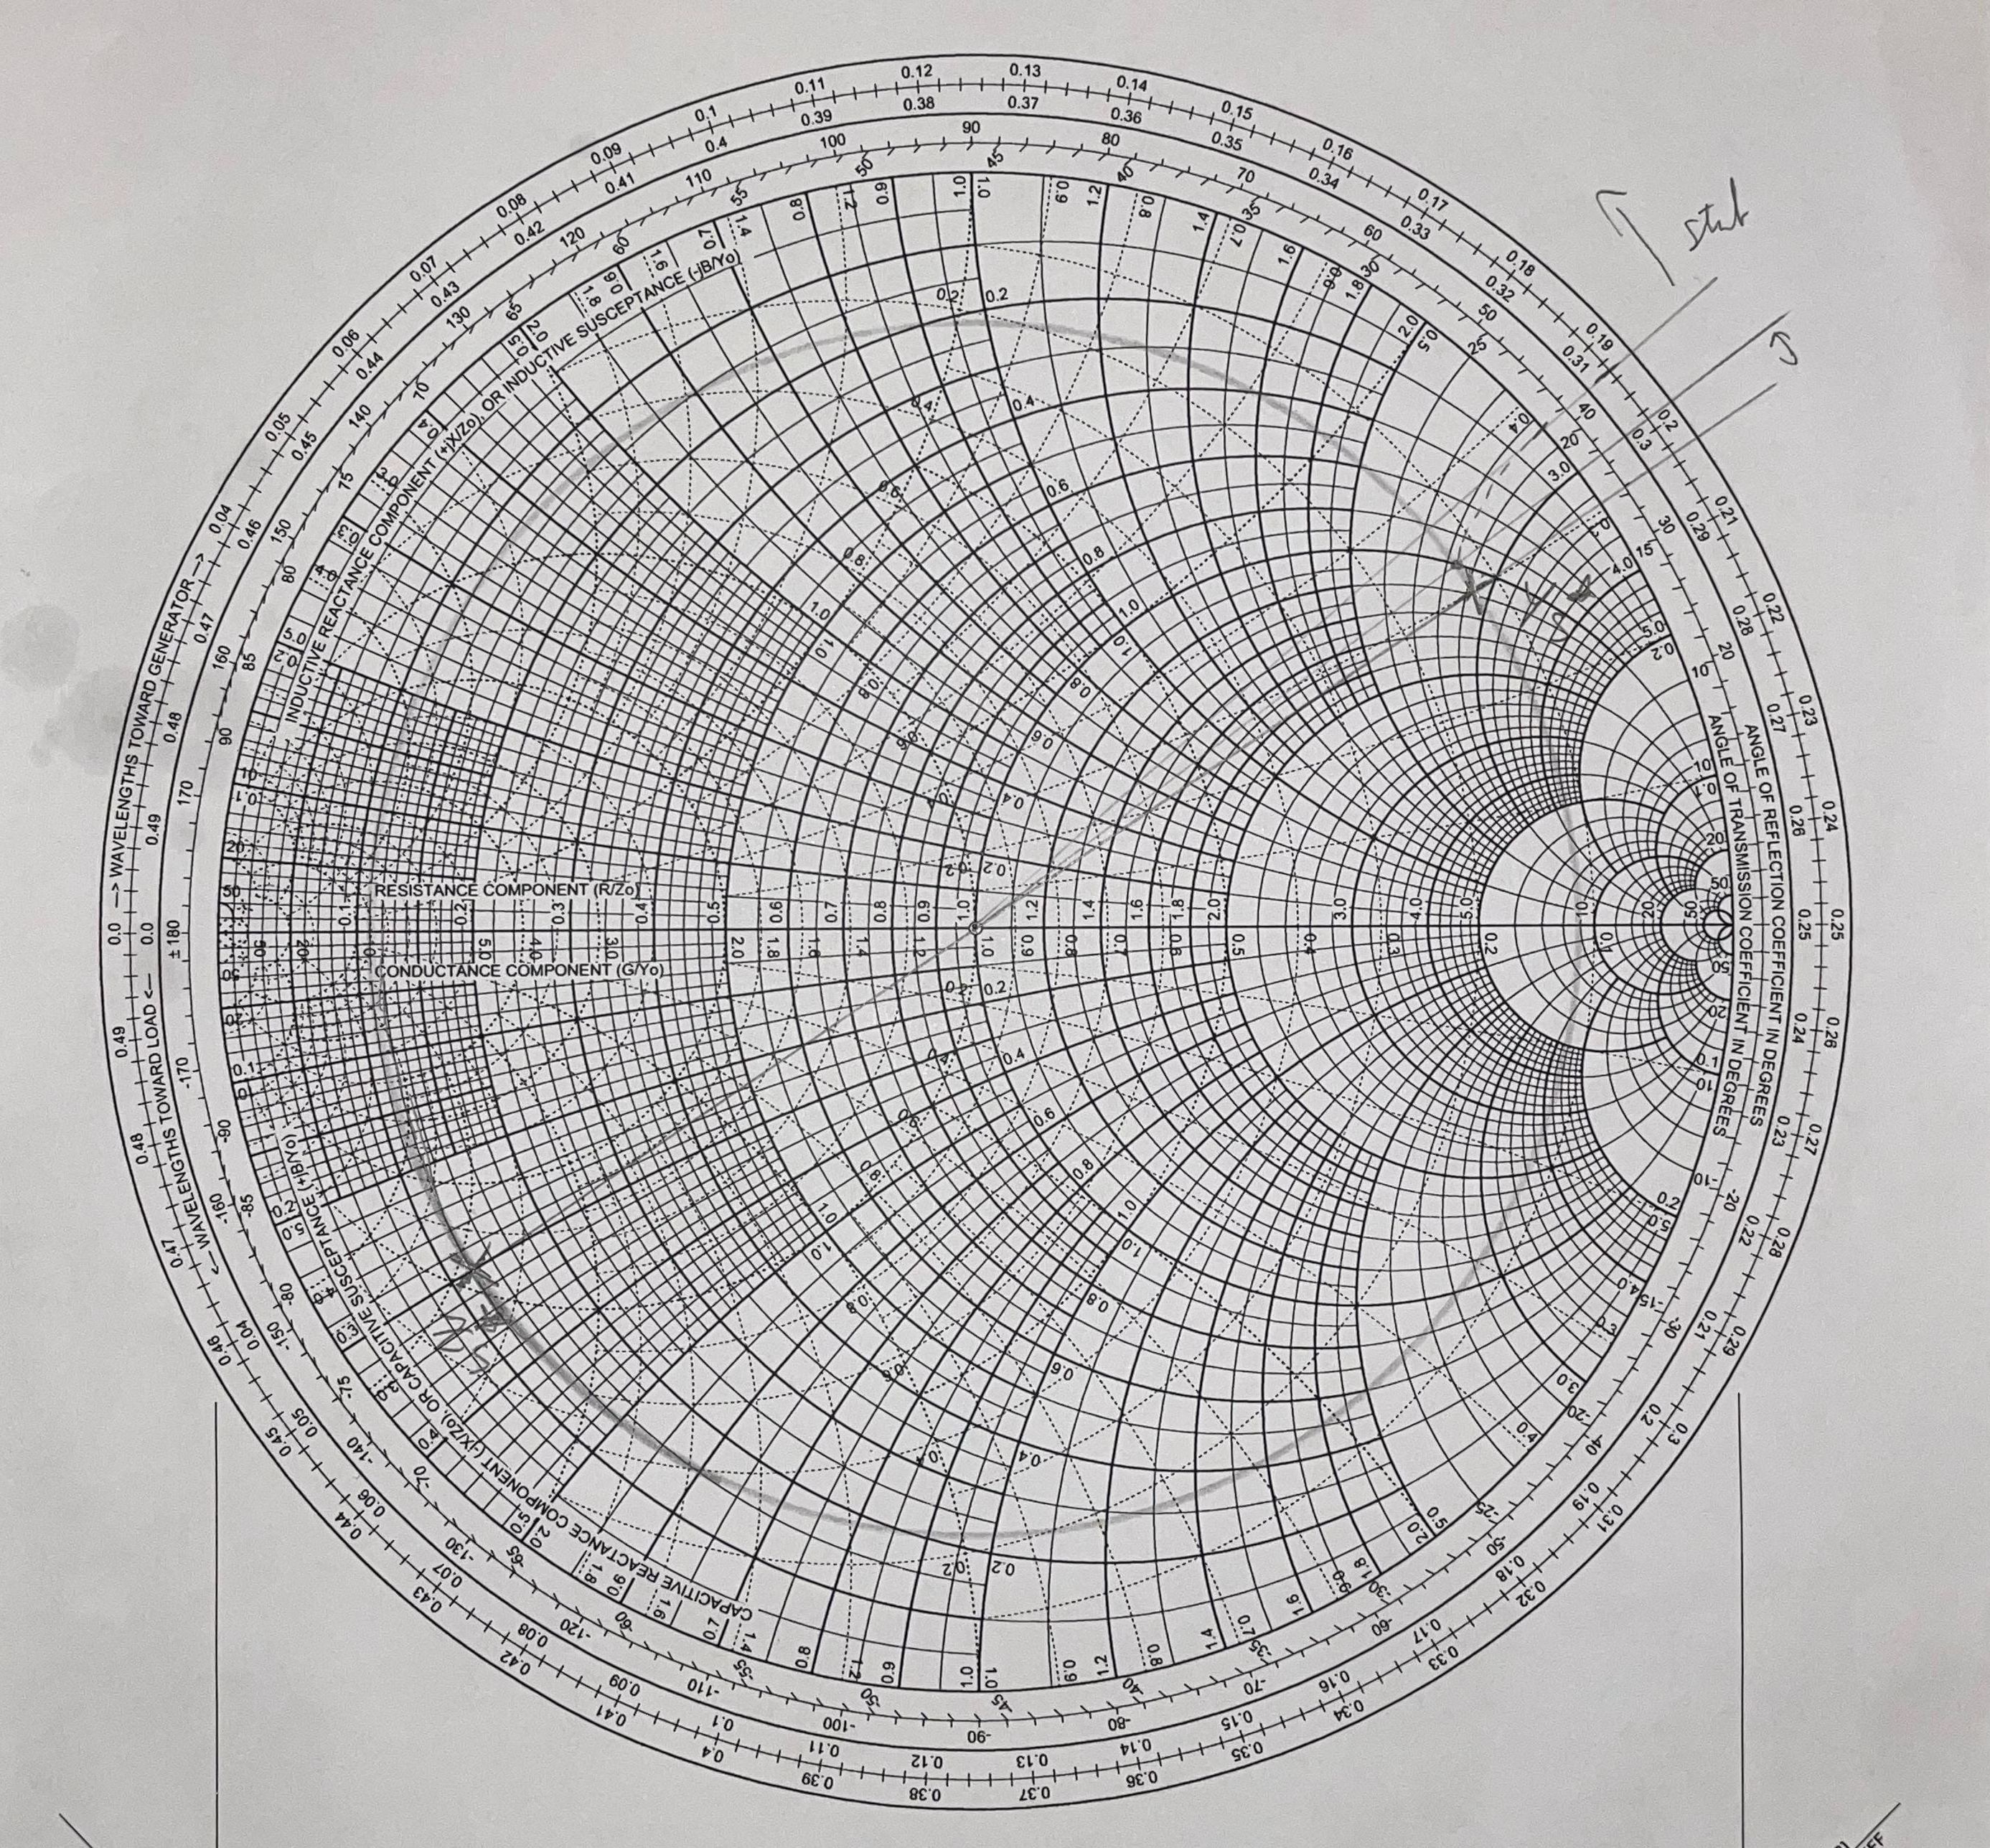
\includegraphics[width=0.4\textwidth]{Images/zs-LS-matching.png}
    \caption{Smith chart for input matching with lines and stubs}
    \label{fig:zs-line-matching}
\end{figure}

The adaptation mesh for the input was done with an open circuit shunt stub and a series line, as shown in Figure \ref{fig:zs_LS_circuit}.

\begin{figure}[H]
    \centering
    \includegraphics[width=0.5\textwidth]{Images/zs_LS_circuit.png}
    \caption{Matching circuit for input with lines and stubs}
    \label{fig:zs_LS_circuit}
\end{figure}

The values obtain from the Smith Chart for the input matching network are shown in Table \ref{tab:MatchingValuesLinesin}.

\begin{table}[H]
    \centering
    \caption{Values of the components for the matching networks using the Smith Chart with lines and stubs.}
    \begin{tabularx}{\textwidth}{>{\centering\arraybackslash}X >{\centering\arraybackslash}X}
        \toprule
        \textbf{Parameter} & \textbf{Value} \\
        \midrule
        $l$     & $0,182\lambda$ \\
        \midrule
        $d$   & $0,007\lambda$ \\
        \bottomrule
    \end{tabularx}
    \label{tab:MatchingValuesLinesin}
\end{table}

\begin{figure}[H]
    \centering
    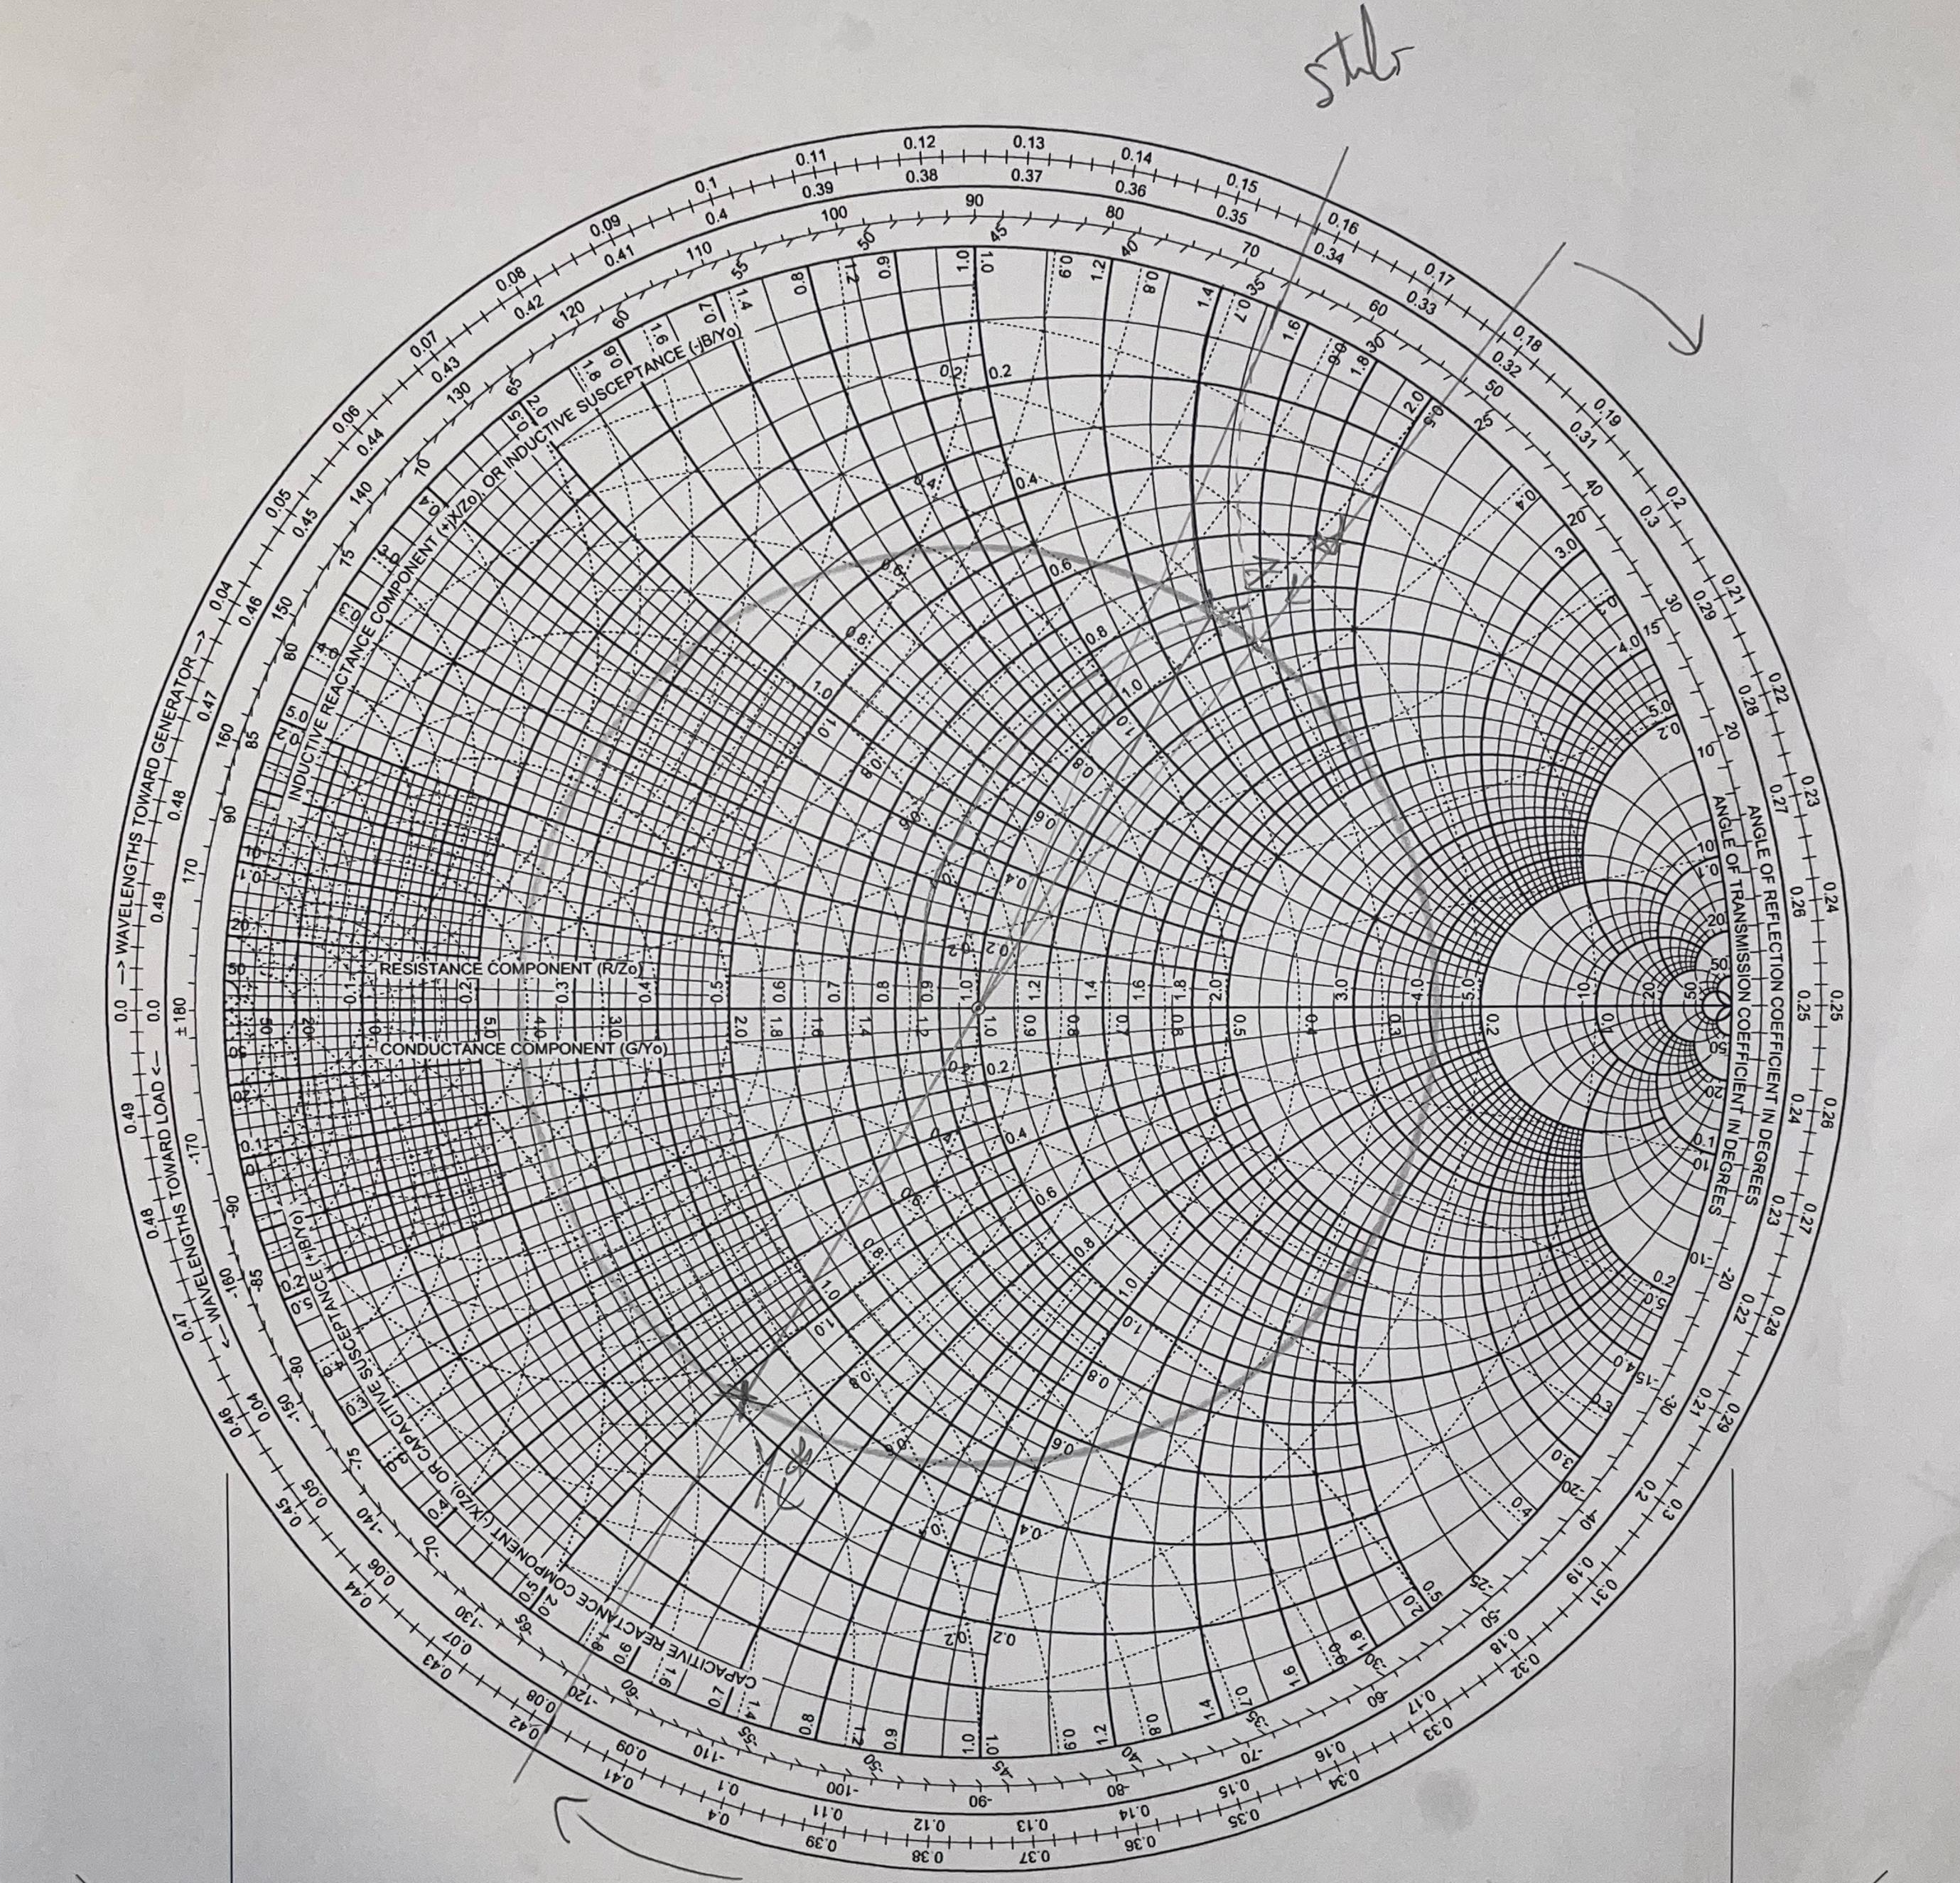
\includegraphics[width=0.4\textwidth]{Images/zl-LS-matching.png}
    \caption{Matching circuit for input with lines and stubs}
    \label{fig:zl-line-matching}
\end{figure}

The adaptation mesh for the output is done with a series line and an open circuit shunt stub as shown in Figure \ref{fig:zl_LS_circuit}.

\begin{figure}[h]
    \centering
    \includegraphics[width=0.5\textwidth]{Images/zl_LS_circuit.png}
    \caption{Matching circuit for output with lines and stubs}
    \label{fig:zl_LS_circuit}
\end{figure}

The values obtain from the Smith Chart for the output matching network are shown in Table \ref{tab:MatchingValuesLinesout}.

\begin{table}[H]
    \centering
    \caption{Values of the components for the matching networks using the Smith Chart with lines and stubs.}
    \begin{tabularx}{\textwidth}{>{\centering\arraybackslash}X >{\centering\arraybackslash}X}
        \toprule
        \textbf{Parameter} & \textbf{Value} \\
        \midrule
        $l$     & $0,169\lambda$ \\
        \midrule
        $d$   & $0,227\lambda$ \\
        \bottomrule
    \end{tabularx}
    \label{tab:MatchingValuesLinesout}
\end{table}

\vspace{0.4cm}
\textbf{Results with analytic approach:}
\vspace{0.4cm}

The expressions used in the Python script to calculate the values of the components are the following \textsuperscript{\cite{Pozar}}:

Considering an impedance $Z$:

\begin{equation}
    Y = G + jB = \frac{1}{Z}
\end{equation}

Where $G$ is the conductance and $B$ is the susceptance and can be calculated as:

\begin{equation}
    G = \frac{R_l(1+t^2)}{R_L^2 + (X_L +Z_0t)^2}
\end{equation}

\begin{equation}
    B = -\frac{R_l^2t-(Z_0-X_Lt)(X_L+Z_0t)}{Z_0[R_L^2 + (X_L +Z_0t)^2]}
\end{equation}

Where $R_l$ is the real part of the impedance, $X_l$ is the imaginary part of the impedance, $Z_0$ is the characteristic impedance of the line and $t$ is the length of the line in wavelengths.

If $R_L$ is different from $Z_0$, the equation for t can be expressed as:

\begin{equation}
    t = \frac{X_L \pm \sqrt{R_L[(Z_0-R_L)^2+X_L^2]/Z_0}}{R_L-Z_0}
\end{equation}

If $R_L = Z_0$, the equation for $t$ can be expressed as:
\begin{equation}
    t = \frac{-X_L}{2Z_0}
\end{equation}

Thus, the solutions for the line lengths $d$ normalized to the wavelength are:

\begin{equation}
    \frac{d}{\lambda} =
    \begin{cases}
        \frac{1}{2\pi}\tan^{-1} t \quad \text{for } t \geq 0 \\
        \frac{1}{2\pi}\left(\pi + \tan^{-1} t\right) \quad \text{for } t < 0
    \end{cases}
    \label{eq:dlength}
\end{equation}

Now to find the open-circuited stub length $l$ normalized to the wavelength, the following equations are used:

\begin{equation}
    \frac{l}{\lambda} = \frac{-1}{2\pi}tan^{-1}\frac{B}{Y_0}
    \label{eq:llength}
\end{equation}

To calculate the wavelength $\lambda$ in the line, the following equation is used:
\begin{equation}
    \lambda = \frac{v}{f}
\end{equation}

And the velocity $v$ in the line is given by:

\begin{equation}
    v = \frac{c}{\sqrt{\epsilon_{eff}}}
\end{equation}

The effective permittivity $\epsilon_{eff}$ is calculated as:

\begin{equation}
    \epsilon_{eff} = \frac{\epsilon_r + 1}{2} + \frac{\epsilon_r - 1}{2}\left(1+\frac{12h}{w}\right)^{-0.5}
\end{equation}
where $w = 1,5 \si{\milli \meter}$ and $h = 800 \si{\micro \meter}$ that correspond to the characteristics of the microstrip line used in the design.


The results obtain from the analytic approach are shown in Table \ref{tab:MatchingValuesLines}. It is possible to observe that the values of the components are very similar to the ones obtained from the Smith Chart, with a difference of less than $5\%$ in all cases. This validates the results obtained from the Smith Chart.

\begin{table}[H]
    \centering
    \caption{Values of the components for the matching networks using the analytic approach with lines and stubs.}
    \begin{tabularx}{\textwidth}{>{\centering\arraybackslash}X >{\centering\arraybackslash}X}
        \toprule
        \textbf{Parameter} & \textbf{Value} \\
        \midrule
        $v$     & $171739780,4465274\,\si{\meter \per \second}$ \\
        \midrule
        $\epsilon_{eff}$     & $3,051410966570356$ \\
        \midrule
        $\lambda$     & $42,90158139038047\,\si{\milli\meter}$ \\
        \midrule
        $l_{in}$     & $8,0649\,\si{\milli\meter}$ \\
        \midrule
        $d_{in}$   & $157,9\,\si{\micro\meter}$ \\
        \midrule
        $l_{out}$     & $7,3823\,\si{\milli\meter}$\\
        \midrule
        $d_{out}$   & $9,6999\,\si{\milli\meter}$\\
        \bottomrule
    \end{tabularx}
    \label{tab:MatchingValuesLines}
\end{table}

The final circuit is shown in Figure \ref{fig:MatchingCircuit-line}, where the input and output matching networks are designed using a combination of transmission lines and stubs.

\begin{figure}[h]
    \centering
    \includegraphics[width=1\textwidth]{Images/LS_matching-circuit.png}
    \caption{Matching circuit for input and output with values.}
    \label{fig:MatchingCircuit-line}
\end{figure}

\subsubsection{Constant Gain circles}

A Python script (Appendix \ref{appendix:python_script}) was made, in line with \cite{Gillermo-Gonzalez}, to calculate the constant gain circles for the input and output matching networks and plot it in the Smith Chart, which are shown in Figure \ref{fig:ConstantGainCircles}. The constant gain circles are used to visualize the gain of the LNA for different source and load impedances. For maximum gain, the source and load impedances should be located on the crosses that represent the maximum gain circles, in this case represent $26,1$ in linear scale or $14,17 \si{\decibel}$.
\begin{figure}[H]
    \centering
    \includegraphics[width=0.4\textwidth]{Images/ConstantGainCircles.png}
    \caption{Constant gain circles for the input matching network.}
    \label{fig:ConstantGainCircles}
\end{figure}

\subsection{Input and output matching networks for Minimum Noise}

After designing the LNA for maximum gain, the next step is to design the input and output matching networks for minimum noise. The goal is to minimize the noise figure ($F$). 

The noise figure is a measure of how much noise the LNA adds to the signal. The lower the noise figure, the better the LNA performs in terms of noise. And it can be defined as \textsuperscript{\cite{Gillermo-Gonzalez}}:

\begin{equation}
    F = \frac{P_{No}}{P_{Ni}G_A}
    \label{eq:NoiseFigure}
\end{equation}

Where $P_{No}$ is the output available noise power, $P_{Ni}$ is the input a<vailable noise power due to $R_n$ and $G_A$ is the available gain of the LNA.

The available gain of the LNA is defined as:
\begin{equation}
    G_A = \frac{P_{So}}{P_{Si}}
    \label{eq:AvailableGain}
\end{equation}

Where $P_{So}$ is the output available signal power and $P_{Si}$ is the input available signal power.

Thus, rewriting equation \ref{eq:NoiseFigure} in terms of the available gain, the noise figure can be expressed as:

\begin{equation}
    F = \frac{P_{Si}/P_{Ni}}{P_{So}/P_{No}} = \frac{SNR_i}{SNR_o}
    \label{eq:NoiseFigure2}
\end{equation}

When working with scattering and noise parameters, the noise figure can be expressed as \textsuperscript{\cite{Gillermo-Gonzalez}}:
\begin{equation}
    F = F_{min} + \frac{r_n}{g_s}|y_s -y_{opt}|^2
    \label{eq:NoiseFigure3}
\end{equation}

Where $F_{min}$ is the minimum noise figure, $r_n$ is the normalized noise resistance, $g_s$ is the normalized source conductance and $y_s$ is the normalized source admittance. The $y_{opt}$ is the optimal source admittance that minimizes the noise figure to the value $F_{min}$.

The following noise parameters where obtain in cadence from the transistor model without any matching network, and compiled in Table \ref{tab:NoiseParameters}.

\begin{table}[H]
    \centering
    \caption{Noise parameters of the transistor.}
    \begin{tabularx}{\textwidth}{>{\centering\arraybackslash}X >{\centering\arraybackslash}X}
        \toprule
        \textbf{Parameter} & \textbf{Value} \\
        \midrule
        $F_{min}$     & $2,171$ \\
        \midrule
        $r_n$     & $9.505\,\si{\ohm}$\\
        \midrule
        $g_s$   & $1.11479037\,\si{\siemens}$ \\
        \midrule
        $y_s$   & $1.11479037+2.54323358j\,\si{\siemens}$ \\
        \midrule
        $y_{opt}$     & $0.02750192+0.00928327j\,\si{\siemens}$\\
        \midrule
        $\Gamma_s$     & $-0.1889065597-0.1585114245j$\\
        \bottomrule
    \end{tabularx}
    \label{tab:NoiseParameters}
\end{table}

Once again a Python script (Appendix \ref{appendix:python_script}) was made to calculate and plot the constant input noise figure circles in the Smith Chart, which are shown in Figure \ref{fig:ConstantNoiseCircles}. The constant noise figure circles are used to visualize the noise figure of the LNA for different source and load impedances. For minimum noise, the source and load impedances should be located on the points that represent the minimum noise figure circles,in this case the crosses, that reoresent $2,2 \si{\decibel}$ corresponding to the minimum noise figure of the transistor.

\begin{figure}[H]
    \centering
    \includegraphics[width=0.4\textwidth]{Images/ConstantNoiseCircles.png}
    \caption{Constant noise figure circles for the input matching network.}
    \label{fig:ConstantNoiseCircles}
\end{figure}    

In order to do the impedance matching for minimum noise, the output reflection coefficient has to be calculated with the following equation \textsuperscript{\cite{Slides}}:
\begin{equation}
    \Gamma_{L} = \left(\frac{s_{22}+(s_{12}s_{21}\Gamma_s)}{1-s_{11}\Gamma_s}\right)^*
    \label{eq:GammaL-noise}
\end{equation}

Now for the sake of simplicity, the reflection coefficients were transformed to the normalized impedances using Equations \ref{eq:Zs} and \ref{eq:Zl}.

In table \ref{tab: noise-impedances} the normalized impedances at the source and load for minimum noise are shown, where the values are calculated using the reflection coefficients obtained in the previous step.

\begin{table}[H]
    \centering
    \caption{Normalized impedances at the source and load for minimum noise.}
    \begin{tabularx}{\textwidth}{>{\centering\arraybackslash}X >{\centering\arraybackslash}X}
        \toprule
        \textbf{Parameter} & \textbf{Value} \\
        \midrule
        $z_{S}$     & $0.652838-0.2203652j$ \si{\ohm} \\
        \midrule
        $z_{L}$     & $1.07281071+0.65421904j$ \si{\ohm}\\
        \bottomrule
    \end{tabularx}
    \label{tab: noise-impedances}
\end{table}

In figure \ref{fig:ZsZl-noise} the normalized impedances at the source and load for minimum noise are shown in the Smith Chart.

\begin{figure}[H]
    \centering
    \includegraphics[width=0.4\textwidth]{Images/ZsZl-noise-smithChart.png}
    \caption{Normalized impedances at the source and load for minimum noise in the Smith Chart.}
    \label{fig:ZsZl-noise}
\end{figure}

Since the Python script (Appendix \ref{appendix:python_script}) for calculating the matching networks has already been verified in the previous section, in this section the matching networks were calculated using it, without the use of the Smith Chart. The equations used in the script are the same as in the previous section, but with the values of the normalized impedances at the source and load for minimum noise.

\subsubsection{Matching with lumped elements for minimum noise}

Using the same matching circuits as in the previous sections, depicted in Figures \ref{fig:MatchingCircuit-input} and \ref{fig:MatchingCircuit-output}, the values of the components were calculated using the Equations \ref{eq:Binside} to \ref{eq:Boutside}.
The results of the matching networks for minimum noise using the analytic approach are shown in Table \ref{tab:MatchingValues-noise}, where the values of the components are calculated based on the input and output impedances of the transistor for minimum noise.
\begin{table}[H]
    \centering
    \caption{Values of the components for the matching networks for minimum noise using the analytic approach.}
    \begin{tabularx}{\textwidth}{>{\centering\arraybackslash}X >{\centering\arraybackslash}X}
        \toprule
        \textbf{Parameter} & \textbf{Value} \\
        \midrule
        $C_{in}$ \quad (shunt)    & $0.5798506944259898\,\si{\pico\farad}$ \\
        \midrule
        $L_{in}$  \quad(series)   & $0.5083089871809204\,\si{\nano\henry}$\\
        \midrule
        $L_{1out}$ \quad (shunt)   & $2.25632568\,\si{\nano\henry}$ \\
        \midrule
        $L_{2out}$ \quad (series)   & $1.36538599\,\si{\nano\henry}$\\
        \bottomrule
    \end{tabularx}
    \label{tab:MatchingValues-noise}
\end{table}

In Figure \ref{fig:MatchingCircuit-noise} the final circuit with the values of the components for minimum noise is shown, where the input and output matching networks are designed using a combination of inductors and capacitors.
\begin{figure}[H]
    \centering
    \includegraphics[width=1\textwidth]{Images/LC-noise-matching-circuit.png}
    \caption{Matching circuit for input and output with final values for minimum noise.}
    \label{fig:MatchingCircuit-noise}
\end{figure}

\subsubsection{Matching lines and stubs for minimum noise}

Using the same matching circuits as in the previous sections, depicted in Figures \ref{fig:zs_LS_circuit} and \ref{fig:zl_LS_circuit}, the values of the components were calculated using the Equations \ref{eq:dlength} to \ref{eq:llength} in the Python script (Appendix \ref{appendix:python_script}).

The results of the matching networks for minimum noise using the analytic approach are shown in Table \ref{tab:MatchingValuesLines-noise}.
\begin{table}[H]
    \centering
    \caption{Values of the components for the matching networks for minimum noise using the analytic approach with lines and stubs.}
    \begin{tabularx}{\textwidth}{>{\centering\arraybackslash}X >{\centering\arraybackslash}X}
        \toprule
        \textbf{Parameter} & \textbf{Value} \\
        \midrule
        $l_{in}$     & $3,21\,\si{\milli\meter}$ \\
        \midrule
        $d_{in}$   & $2,13\,\si{\milli\meter}$ \\
        \midrule
        $l_{out}$     & $3,87\,\si{\milli\meter}$\\
        \midrule
        $d_{out}$   & $2,47\,\si{\milli\meter}$\\
        \bottomrule
    \end{tabularx}
    \label{tab:MatchingValuesLines-noise}
\end{table}

The final circuit with the values of the components for minimum noise is shown in Figure \ref{fig:MatchingCircuit-line-noise}, where the input and output matching networks are designed using a combination of transmission lines and stubs.

\begin{figure}[H]
    \centering
    \includegraphics[width=1\textwidth]{Images/LS-noise-matching-circuit.png}
    \caption{Matching circuit for input and output with values for minimum noise.}
    \label{fig:MatchingCircuit-line-noise}
\end{figure}


\subsection{Gain-Noise Optimization}

To optimize the LNA for both gain and noise, a trade-off between the two parameters is necessary. The goal is to find a balance between the maximum gain and the minimum noise figure. To obtain this result the input gain circles and the input noise circles were plotted in the Smith Chart and analyzed, the plot is shown in Figure \ref{fig:GainNoiseOptimization}. 

\begin{figure}[H]
    \centering
    \includegraphics[width=0.4\textwidth]{Images/GainNoiseOptimization.png}
    \caption{Gain and noise circles for the input matching network.}
    \label{fig:GainNoiseOptimization}
\end{figure}
The intersection of the gain and noise circles represents the optimal point for the LNA, where the gain is maximized ($G = 21$) while the noise figure is minimized ($F = 3 \si{\decibel}$).

In table \ref{tab:GainNoiseOptimization} the values of the intersection points of the 21 gain circle and the 3 dB noise figure circle are shown, where the values were calculated using the Python script (Appendix \ref{appendix:python_script}).

\begin{table}[H]
    \centering
    \caption{Values of the intersection points of the gain and noise circles.}
    \begin{tabularx}{\textwidth}{>{\centering\arraybackslash}X >{\centering\arraybackslash}X}
        \toprule
        \textbf{Parameter} & \textbf{Value} \\
        \midrule
        $\Gamma_{A1}$     & $-0.30695536-0.15142555j$ \si{\ohm} \\
        \midrule
        $\Gamma_{A2}$     & $-0.22141437-0.27183862j$ \si{\ohm} \\
        \midrule
        $z_{A1}$     & $0.51000409-0.17495104j$ \si{\ohm} \\
        \midrule
        $z_{A2}$     & $0.56016594-0.34723135j$ \si{\ohm}\\
        \bottomrule
    \end{tabularx}
    \label{tab:GainNoiseOptimization}
\end{table}

For the following calculations $\Gamma_s = \Gamma_{A1}$ and $z_{A1} = z_s$ will be used.

Once again in order do obtain a bilateral matching network, the output reflection coefficient has to be calculated with the equation  \ref{eq:GammaL-noise}. Withthe reflection coefficient value, it is possible to obtain the normalized impedance at the load using the equation \ref{eq:Zl}.

In table \ref{gain-noise-impedances} the normalized impedances at the source and load and the reflection coefficients for gain-noise optimization are shown.

\begin{table}[H]
    \centering
    \caption{Normalized impedances at the source and load for gain-noise optimization.}
    \begin{tabularx}{\textwidth}{>{\centering\arraybackslash}X >{\centering\arraybackslash}X}
        \toprule
        \textbf{Parameter} & \textbf{Value} \\
        \midrule
        $z_{S}$     & $0.51000409-0.17495104j$ \si{\ohm} \\
        \midrule
        $z_{L}$     & $0.95353092+0.74623035j$\si{\ohm}\\
        \midrule
        $\Gamma_{S}$     & $-0.30695536-0.15142555j$\\
        \midrule
        $\Gamma_{L}$     & $0.10657803+0.34127875j$\\
        \bottomrule
    \end{tabularx}
    \label{gain-noise-impedances}
\end{table}

In Figure \ref{fig:ZsZl-gain-noise} the normalized impedances at the source and load for gain-noise optimization are shown in the Smith Chart.

\begin{figure}[H]
    \centering
    \includegraphics[width=0.4\textwidth]{Images/gain-noise-SC.png}
    \caption{Normalized impedances at the source and load for gain-noise optimization in the Smith Chart.}
    \label{fig:ZsZl-gain-noise}
\end{figure}

\subsubsection{Matching with lumped elements for gain-noise optimization}

Using the same matching circuits as in the previous sections, depicted in Figures \ref{fig:MatchingCircuit-input} and \ref{fig:MatchingCircuit-output}, the values of the components were calculated using the Equations \ref{eq:Binside} to \ref{eq:Boutside} in the Python script (Appendix \ref{appendix:python_script}).

The results of the matching networks for gain-noise optimization using the analytic approach are shown in Table \ref{tab:MatchingValues-gain-noise}.

\begin{table}[H]
    \centering
    \caption{Values of the components for the matching networks for gain-noise optimization using the analytic approach.}
    \begin{tabularx}{\textwidth}{>{\centering\arraybackslash}X >{\centering\arraybackslash}X}
        \toprule
        \textbf{Parameter} & \textbf{Value} \\
        \midrule
        $C_{in}$ \quad (shunt)    & $0.779402735\,\si{\pico\farad}$ \\
        \midrule
        $L_{in}$  \quad(series)   & $0.64596288\,\si{\nano\henry}$\\
        \midrule
        $L_{1out}$ \quad (shunt)   & $9.00487954\,\si{\nano\henry}$ \\
        \midrule
        $L_{2out}$ \quad (series)   & $1.06497606\,\si{\nano\henry}$\\
        \bottomrule
    \end{tabularx}
    \label{tab:MatchingValues-gain-noise}
\end{table}

In Figure \ref{fig:MatchingCircuit-gain-noise} the final circuit with the values of the components for gain-noise optimization is shown.

\begin{figure}[H]
    \centering
    \includegraphics[width=1\textwidth]{Images/gain-noise-final-circuit.png}
    \caption{Matching circuit for input and output with final values for gain-noise optimization.}
    \label{fig:MatchingCircuit-gain-noise}
\end{figure}

\subsubsection{Matching lines and stubs for gain-noise optimization}

Once again were used the same matching circuits as in the previous sections, depicted in Figures \ref{fig:zs_LS_circuit} and \ref{fig:zl_LS_circuit}, the values of the components were calculated using the Equations \ref{eq:dlength} to \ref{eq:llength} in the Python script (Appendix \ref{appendix:python_script}).

The results of the matching networks for gain-noise optimization using the analytic approach are shown in Table \ref{tab:MatchingValuesLines-gain-noise}.

\begin{table}[H]
    \centering
    \caption{Values of the components for the matching networks for gain-noise optimization using the analytic approach with lines and stubs.}
    \begin{tabularx}{\textwidth}{>{\centering\arraybackslash}X >{\centering\arraybackslash}X}
        \toprule
        \textbf{Parameter} & \textbf{Value} \\
        \midrule
        $l_{in}$     & $4,299\,\si{\milli\meter}$ \\
        \midrule
        $d_{in}$   & $2,605\,\si{\milli\meter}$ \\
        \midrule
        $l_{out}$     & $4,462\,\si{\milli\meter}$\\
        \midrule
        $d_{out}$   & $10,511\,\si{\milli\meter}$\\
        \bottomrule
    \end{tabularx}
    \label{tab:MatchingValuesLines-gain-noise}
\end{table}

The final circuit with the values of the components for gain-noise optimization is shown in Figure \ref{fig:MatchingCircuit-line-gain-noise}, where the input and output matching networks are designed using a combination of transmission lines and stubs.

\begin{figure}[H]
    \centering
    \includegraphics[width=1\textwidth]{Images/LS-gain-noise-matching-circuit.png}
    \caption{Matching circuit for input and output with values for gain-noise optimization.}
    \label{fig:MatchingCircuit-line-gain-noise}
\end{figure}